\documentclass{beamer}
\usepackage{xcolor}

% \usepackage{beamerthemesplit} // Activate for custom appearance

\title{On (mod $n$) Spirals}
\author{Andrew R. Reiter (Veracode, Inc.)\\
Robin Young (UMASS-Amherst)}
\date{\today}

\theoremstyle{mydef}
%\newtheorem{definition}{}
\newtheorem{conj}{Conjecture}[section]
\newtheorem{thm}{Theorem}[section]

\begin{document}

\frame{\titlepage}

%\section[Outline]{}
%\frame{\tableofcontents}


\frame
{
  \frametitle{Polar Vortex!}

  \begin{itemize}
  \item Cold Winter\\
  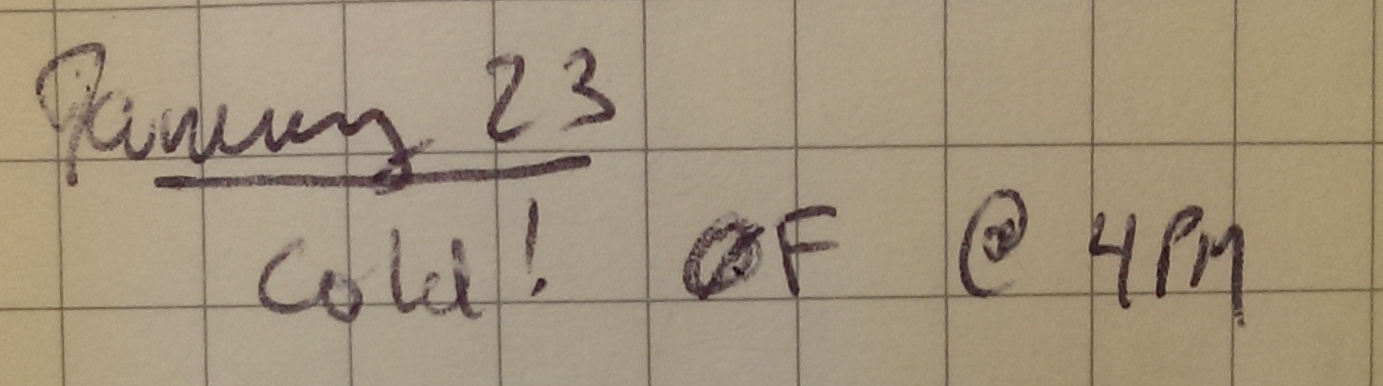
\includegraphics[scale=.15]{images/PolarVortex1.png}
  \item Led to being sick and in bed for ~2 weeks... 
  \item What to do? MATH!... or at least play with numbers
  \end{itemize}  
}



\frame
{
  \frametitle{Orderly Doodling}
 \[
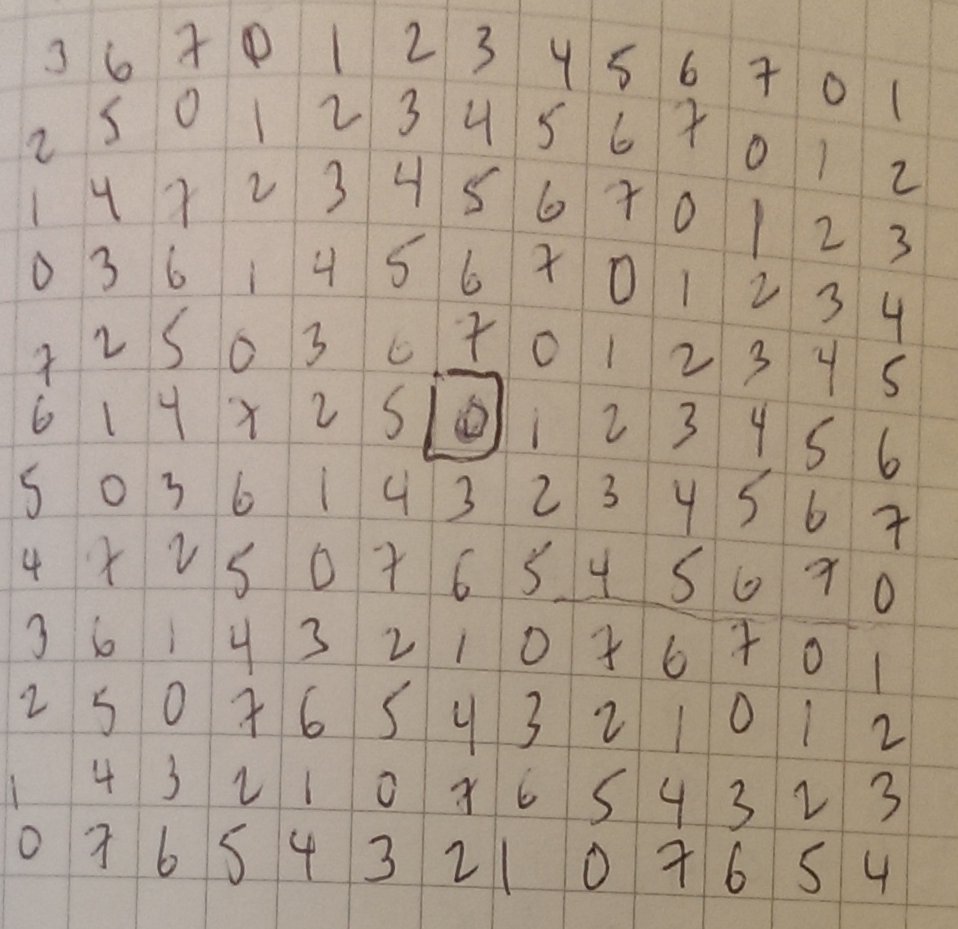
\includegraphics[scale=.15]{images/mod8.png}\quad
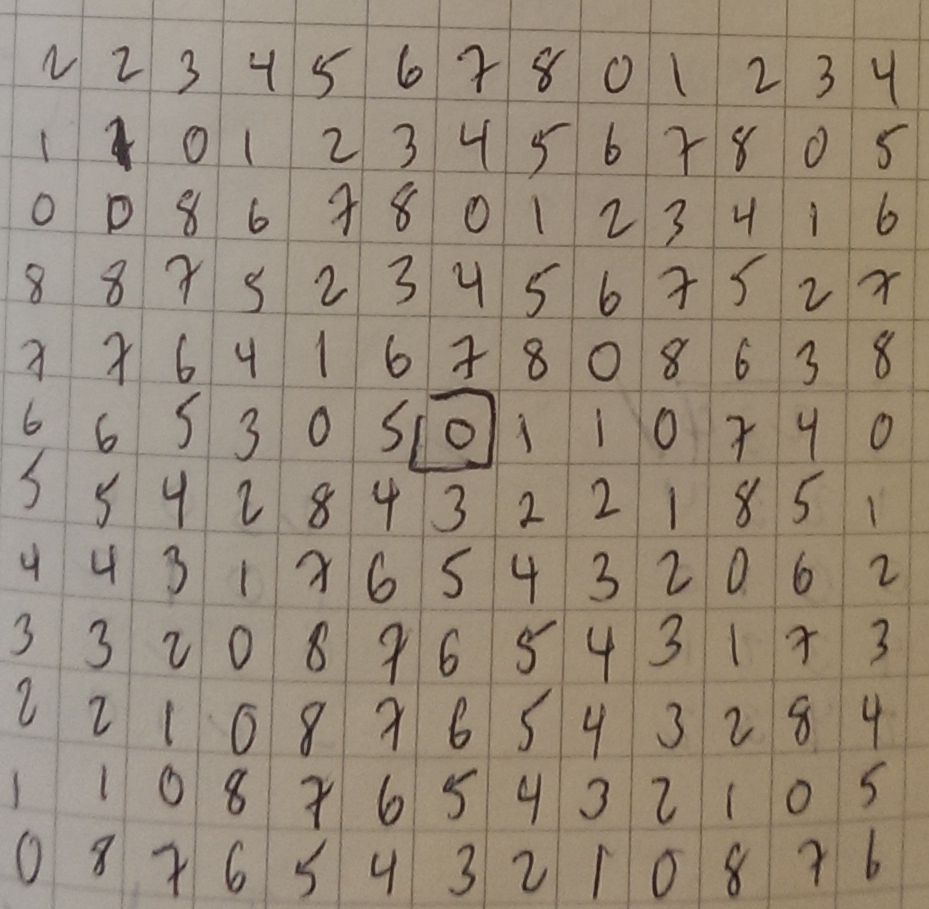
\includegraphics[scale=.15]{images/mod9.png}
\]
}


\frame
{
  \frametitle{What is the process?}
  Select an integer $n \ge 2$, say $n = 3$, noting $\mathbb{Z}_3 = \{ 0, 1, 2\}$
  \begin{center}
  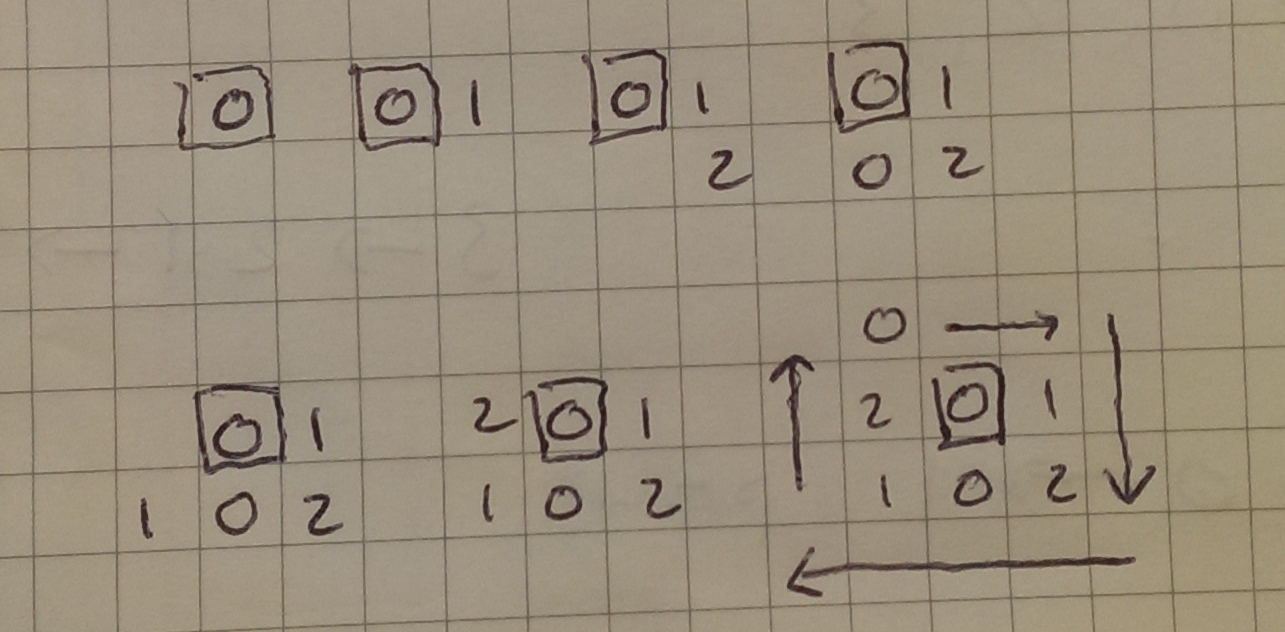
\includegraphics[scale=.1]{images/mod3move.png}
  \end{center}
\tiny
\[  \begin{array}{c}
\boxed{0}
\end{array} 
\rightarrow
%
\begin{array}{cc}
\boxed{0} & 1 \\
\  & \ 
\end{array}
\rightarrow
\begin{array}{cc}
\boxed{0} & 1 \\
\  & 2
\end{array}
\rightarrow
\begin{array}{cc}
\boxed{0} & 1 \\
0 & 2
\end{array}
\rightarrow
\]

\[
\begin{array}{ccc}
\  & \boxed{0} & 1 \\
1 & 0 & 2
\end{array}
\rightarrow
\begin{array}{ccc}
2 & \boxed{0} & 1 \\
1 & 0 & 2
\end{array}
\rightarrow
\begin{array}{ccccc}
\  & 0 & \cdot  & \cdot & \cdot \\
\  & 2 & \boxed{0} & 1 & \cdot \\
\  & 1 & 0 & 2 & \cdot \\
\cdot & \cdot & \cdot & \cdot & \cdot
\end{array}
\]
Formally,
\[
  l_j^* = j-1 \!\!\!\pmod n \quad\text{at site}\quad l_j.
\]

}



\frame
{
  \frametitle{Patterns Seemed Interesting}
\[
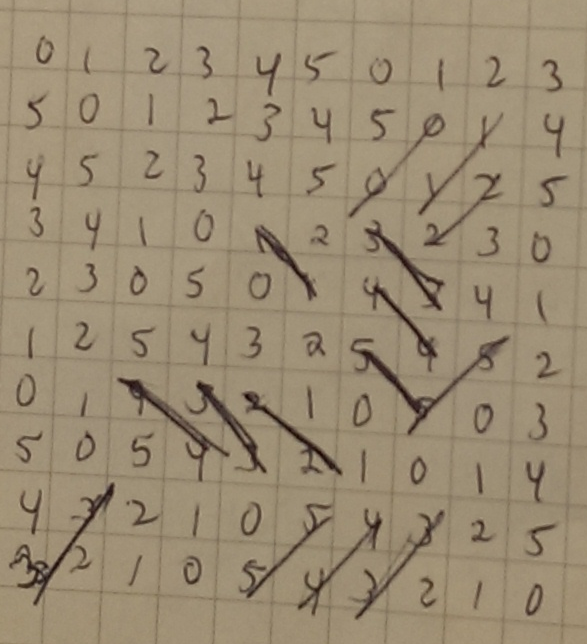
\includegraphics[scale=.2]{images/mod6scratch.png}\quad
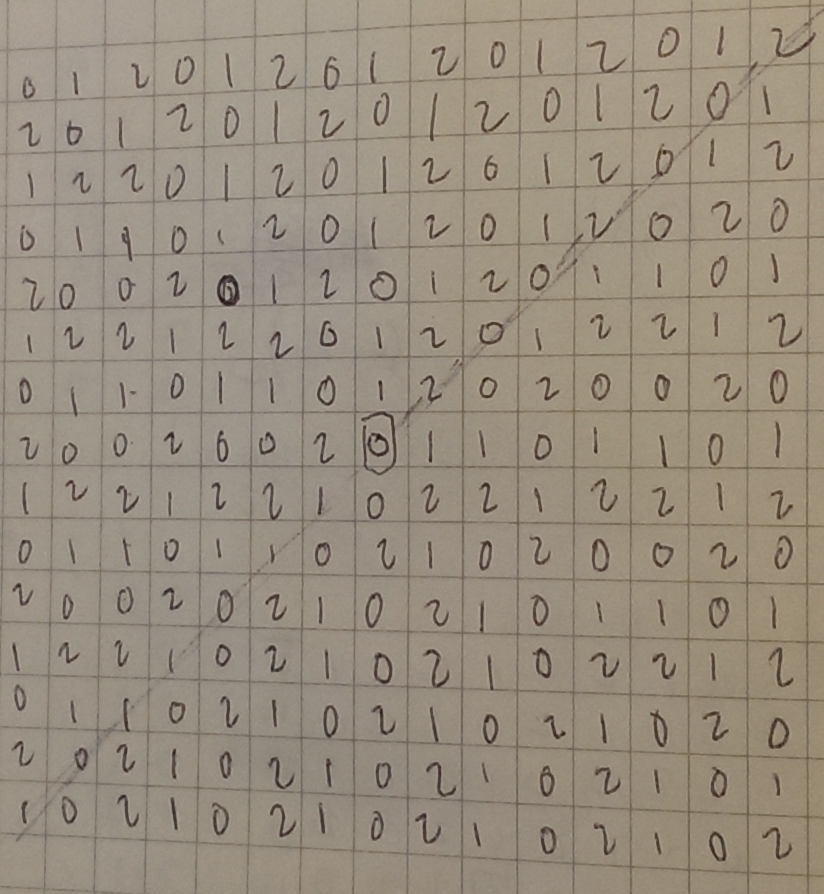
\includegraphics[scale=.15]{images/bigmod3hand.png}
\]

...want larger spirals!
}



\frame
{
  \frametitle{Desire to Automate}

  \begin{columns}
    \begin{column}{.5\textwidth}
     \begin{block}{
     
     \color{black}
  \begin{itemize}
       \color{black}

  \item Want bigger spirals, but...tedious when writing out.
  \item Write a program!
    \end{itemize} 
}
% Your text here
    \end{block}
    \end{column}
    \begin{column}{.5\textwidth}
    \begin{block}{}
% Your image included here
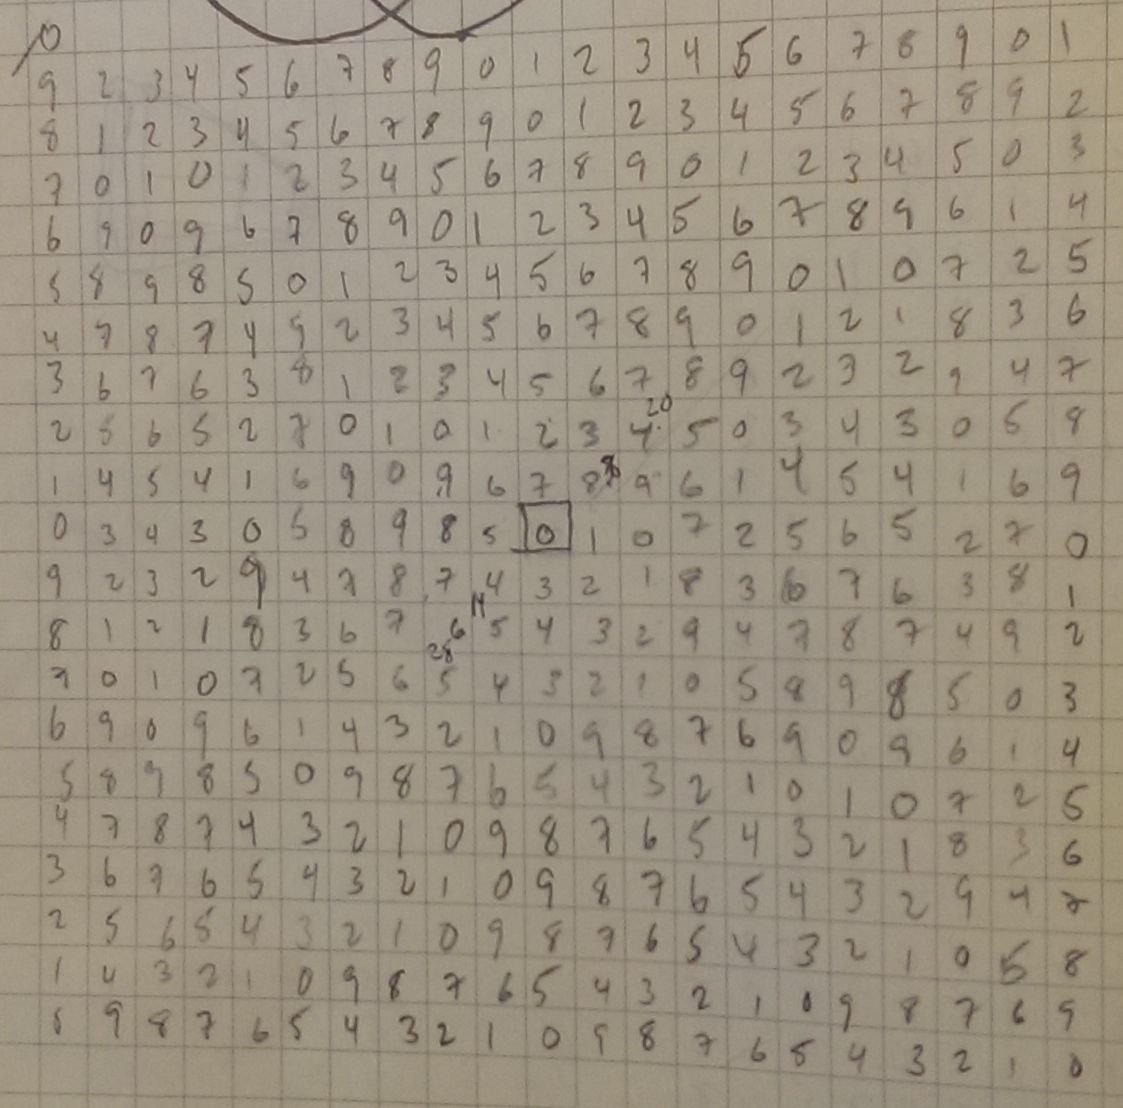
\includegraphics[scale=.13]{images/bigmod10.png}
    \end{block}
    \end{column}
  \end{columns}
  }


\frame
{
\frametitle{Desire for Definition}

\begin{itemize} 
\item A \emph{complete spiral} occurs when form a square and last value assigned is $l^*_i = n-1$
\begin{itemize}
\item Denote the first complete spiral achieved by $Ond^1_n$; 
\item subsequent complete spirals are denoted $Ond^k_n$, $k = 2,3,\dots$.  
\item  The word ``ond'' is ``spiral'' in Swahili.
\end{itemize}
\item The number of times $\mathbb{Z}_n$ is used in order to complete the $k^{th}$ square is the \emph{iteration count}. 
\end{itemize}
}

\section{Visuals}
\frame
{
  \frametitle{Visualize the patterns}
  Realize generated $Ond_n^k$ as grayscale graphical images
  
  The map $f : \mathbb{Z}_n \to \mathbb{Z}_{256}$ is defined by a scaled floor function,
\[
   f(j) = \alpha j, \quad \text{where} \quad
   \alpha = \left\lfloor \frac{255}n \right\rfloor
\]
}

\subsection{Square Lattice}
\frame
{
  \frametitle{Square Lattice}

  \[
 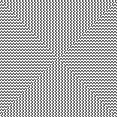
\includegraphics[scale=.8]{images/Ond-N3-k39.png}\quad
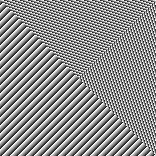
\includegraphics[scale=.5]{images/Ond-N8-k39.png}\quad
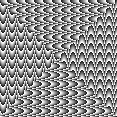
\includegraphics[scale=.5]{images/Ond-N9-k39.png}
\]
  \[
  Ond_3^{39}\quad Ond_{8}^{39}\quad Ond_{9}^{39} \text{ respectively}
  \]
}

\frame
{
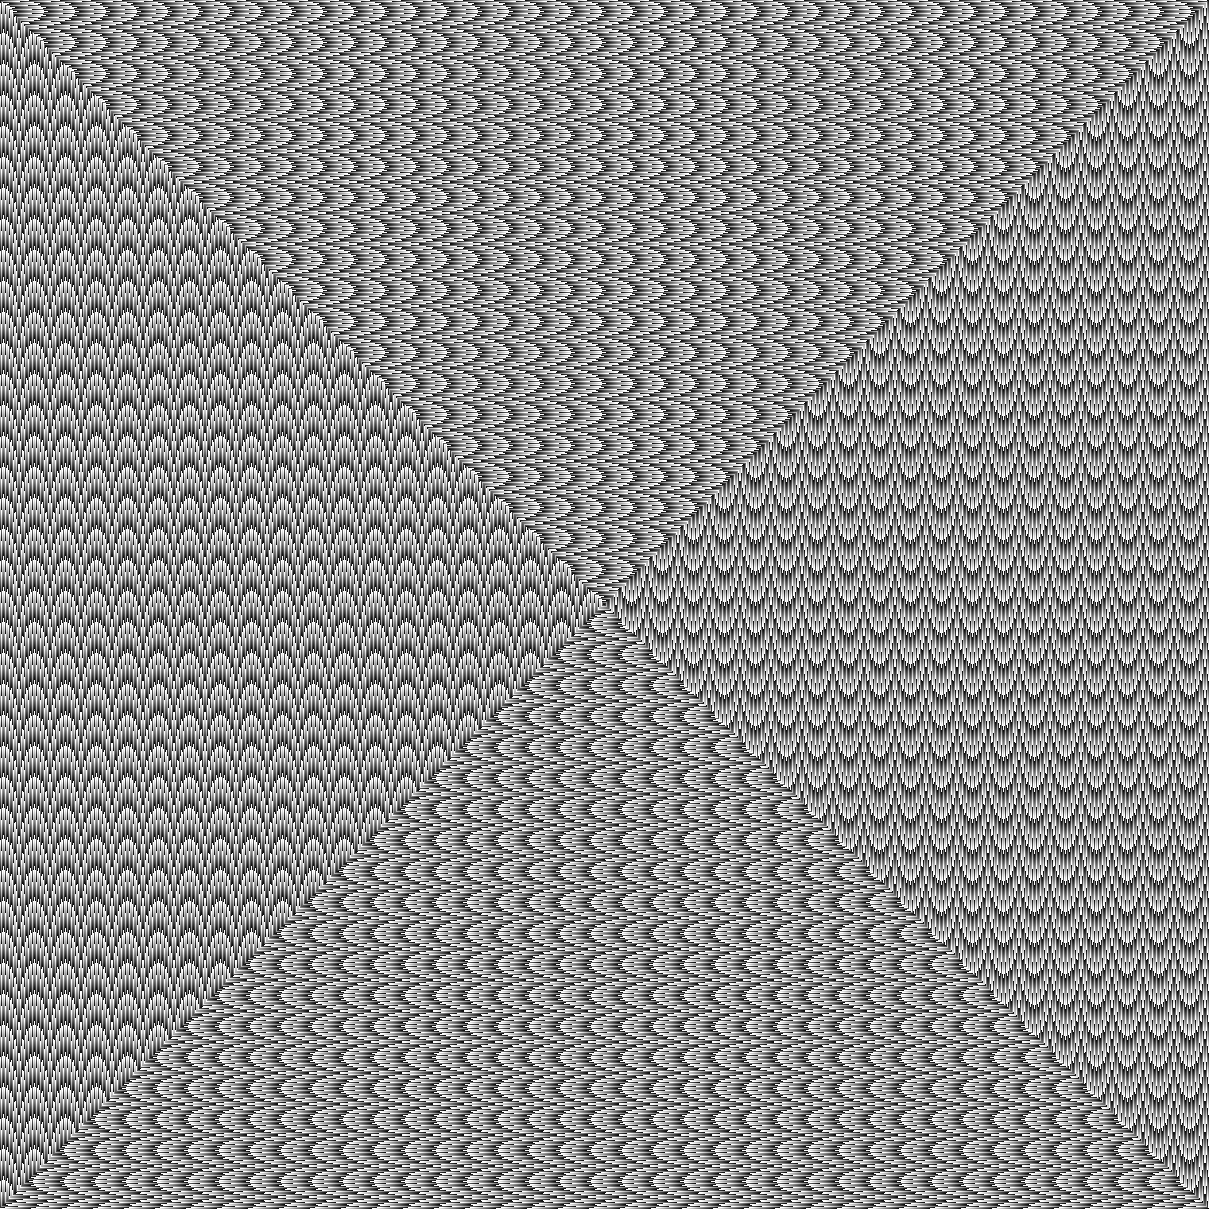
\includegraphics[scale=.25]{images/Ond-N31-k39.png}
}


\frame
{
  \frametitle{Automation to Conjecture}
  
  \begin{itemize}
  \item Is there some general pattern to square sizes?
  \item Side lengths for $Ond_8^{39} > Ond_9^{39}$
  
  156 and 117, respectively  
  \item Can I use $(n, k, ?)$ to determine this?
  \item Using data generated from forming 
  \end{itemize}
}

\frame
{
  \frametitle{}
  \begin{thm}%[Length of Sides of $Ond^k_n$]
\label{lenthm}
\footnotesize
Let $s$ denote the greatest square divisor of $n$.
The complete spiral $Ond^k_n$ has the following structure:
\begin{enumerate}[(i)]
\item If $\lambda$ is the length of the sides of $Ond^k_n$, then
\begin{equation}
  \lambda = \frac{kn}{\sqrt{s}}.
\label{lambda}
\end{equation}
\item If $\xi$ is the iteration count of $Ond^k_n$, then
\begin{equation}
  \xi = \frac{k^2n}{s}.  
\label{xi}
\end{equation}
\item If $l_{max} \in L$ is the last lattice point in the complete
  spiral $Ond^k_n$, then $l_{max}$ is either the top-right corner or
  bottom-left corner of the square.  If both $n$ and $k$ are odd, then
  $l_{max}$ will be the top-right corner of $Ond^k_n$.  In all other
  cases, $l_{max}$ will be the bottom-left corner.
\end{enumerate}
\end{thm}
See paper for proof.
}

\frame
{
  \frametitle{Greatest Perfect Square Divisor of $n$}
  
  Write down $Ond_n^1$, determine side length, solve $\lambda = \frac{n}{\sqrt{s}}$ for $s$.
}


\subsection{Other Shapes}
\frame
{
  \begin{itemize}
  \item Think of geometrically as filling an area
  \item Extend square $Ond$ to $d$-dim hypercube by looking at $n \vert \lambda^d$
  \item Difficult to visualize
  \end{itemize}
}
  
\frame
{
  \frametitle{Centered Hexagons}
  \begin{itemize}
  \item Centered hexagonal numbers are $H_d = 3d(d+1)+1$
  \item Investigate $n \vert H_d$
  \end{itemize}
\[
  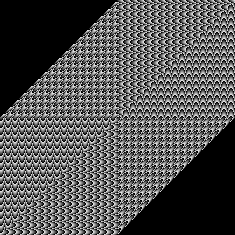
\includegraphics[scale=.45]{images/hex-sp-N7-k34.png}\quad
  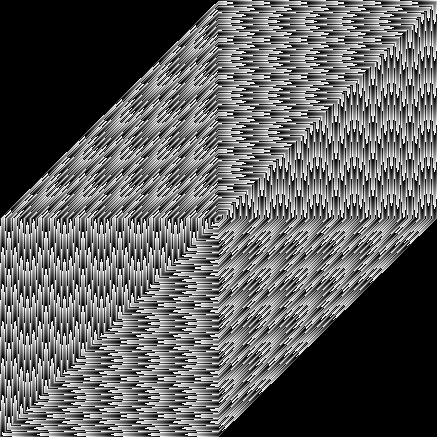
\includegraphics[scale=.25]{images/hex-sp-N37-k12.png}
\]
  GRAPHIC
}

\frame
{
  \frametitle{Triangles}
  \begin{itemize}
  \item Triangle numbers are $T_d = \frac{d(d+1)}{2}$
    \item Investigate $n \vert T_d$
 \end{itemize}
  GRAPHIC
}

\section{Conclusion}
\frame{
\frametitle{So what is all this?}
\begin{itemize}
\item Opportunity to show how one can impose definitions and ideas to patterns you see.
\item From here you can prove conjectures based on observations by playing with these ideas.
\item Learn to generalize and apply ideas to different contexts
\end{itemize}
}
\frame
{
  \frametitle{Things to Explore}
  \begin{itemize}
  \item Other 2 dimensional lattice shapes
  \item Non-hypercube shapes in $>2$ dimensions
  \item Adding $Ond$'s (see visualizations)
  \item Random $Ond$: Select $n_0$ from some distribution, cycle through $\mathbb{Z}_{n_0}$ once, choose $n_1$,  cycle through $\mathbb{Z}_{n_1}$, ...
  \end{itemize}
}
\frame
{
  \frametitle{Thank You!}
  We invite you to please take a paper if you are interested in this topic. For code and visualizations, please go to https://github.com/cwcomplex/modNspirals
  \begin{itemize}
  \item Robin Young of UMASS-Amherst
  \item Veracode, Inc -- Hackathon!
  \item Jared Carlson of Veracode
  \end{itemize}
  Contact: areiter@veracode.com, young@math.umass.edu
}
\end{document}
